\documentclass[a4paper, 12pt]{article}%тип документа

%отступы
\usepackage[left=2cm,right=2cm,top=2cm,bottom=3cm,bindingoffset=0cm]{geometry}

%Русский язык
\usepackage[T2A]{fontenc} %кодировка
\usepackage[utf8]{inputenc} %кодировка исходного кода
\usepackage[english,russian]{babel} %локализация и переносы

%Вставка картинок
\usepackage{graphicx}
\graphicspath{{pictures/}}
\DeclareGraphicsExtensions{.pdf,.png,.jpg}

%Графики
\usepackage{multirow}
\usepackage{pgfplots}
\pgfplotsset{compat=1.9}

%Римские цифры
\newcommand{\RNumb}[1]{\uppercase\expandafter{\romannumeral #1\relax}}

%Математика
\usepackage{amsmath, amsfonts, amssymb, amsthm, mathtools}

%Заголовок
\author{Богданов Александр \\
	Б05-003}
\title{\textbf{Работа 5.1.2 \\ 
		Исследование эффекта Комптона}}

\begin{document}

\maketitle

\textbf{Цель работы:}  исследовать энергетический спектр $\gamma$-квантов,  рассеянных на графите,  определить энергию рассеянных $\gamma$-квантов в зависимости от угла рассеяния,  определить энергию покоя частиц,  на которых происходит комптоновское рассеяние.

\textbf{В работе используются:} источник излучения,  графитовая мишень,  лимб, сцинтилляционный счётчик,  фотоэлектронный умножитель (ФЭУ),  ЭВМ.\\

\textbf{Теоретические положения:}\\\par

	Эффект Комптона - увеличение длины волны рассеянного излучения по сравнению с падающим. Он интерпретируется как результат упругого соударения двух частиц - $\gamma$-кванта и свободного электрона. \par
	
	Пусть электрон до соударения покоился,  а  $\gamma$-квант имел начальную энергию $\hbar \omega_0$ и импульс $\hbar \omega_0/c$.  После соударения электрон приобретает энергию $\gamma mc^2$,  где $\gamma = (1 - \beta^2)^{-1/2}$,  $\beta = v/c$,  а  $\gamma$-квант рассеивается на некоторый угол $\theta$ по отношению к первоначальному направлению движения.  Энергия и импульс $\gamma$-кванта становятся соотвественно равными  $\hbar \omega_0$ и $\hbar \omega_0/c$.  Тогда для рассматриваемого процесса законы сохранения энергии и импульса:

\[ mc^2 + \hbar \omega_0 = \gamma mc^2 + \hbar \omega_1\]

\[\frac{\hbar \omega_0}{c} = \gamma mv \cos \varphi + \frac{\hbar \omega_1}{c} \cos \theta\]

\[\gamma mv \sin \varphi = \frac{\hbar \omega_1}{c} \sin \theta\]

Решая совместно эти уравнения,  получаем изменение длины рассеянного излучения:

    \[\triangle \lambda = \lambda_1 - \lambda_0 = \frac{h}{mc}(1 - \cos \theta) = \Lambda_k(1 - \cos \theta),\]
где $\Lambda_k = \frac{h}{mc} = 2.42 \cdot 10^{-10}$ см - комптоновская длина волны электрона. \par

Преобразуем выражение от длин волн к энергии $\gamma$-квантов:

\[\frac{1}{\varepsilon(\theta)} - \frac{1}{\varepsilon_0} = 1 - \cos \theta,\]
где $\varepsilon_0 = E_0/(mc^2)$ - энергия $\gamma$-квантов, падающих на рассеиватель (в единицах $mc^2$),  $\varepsilon(\theta)$ - выраженная в тех же единицах энергия квантов, испытавших комптоновское рассеяния на угол $\theta$, $m$ - масса электрона.\\

\textbf{Экспериментальная установка:}\\\par

\begin{figure}[h]
	\begin{center}
		\begin{minipage}[h]{0.48\linewidth}
			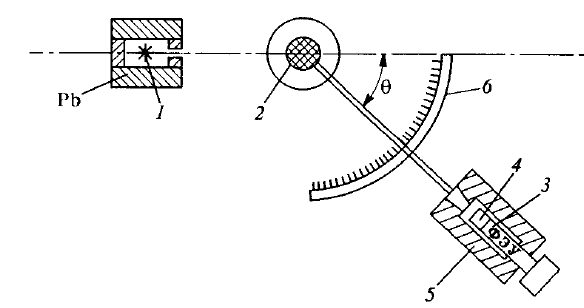
\includegraphics[width=1\linewidth]{Схема1.PNG}
		\end{minipage}
		\hfill 
		\begin{minipage}[h]{0.48\linewidth}
			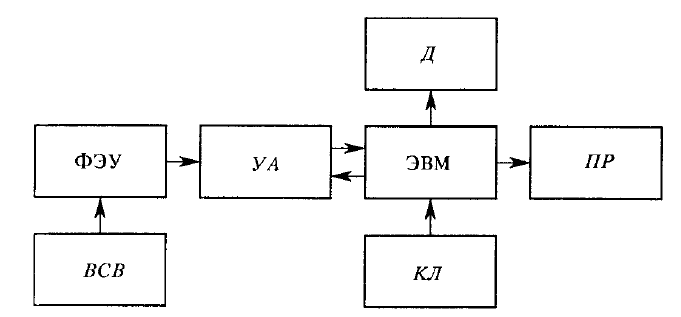
\includegraphics[width=1\linewidth]{Схема2.PNG}
		\end{minipage}
	\end{center}
\end{figure}

Источником излучения служит $^{137}$Cs (1),  испускающий  $\gamma$-кванты с энергией 662 кэВ.  Узкий пучок после коллиматора попадает на графитовую мишень (2). Кванты,  испытавшие комптоновское рассеяния в мишени,  регистрируются сцинтилляционным счетчиком и проходят на ФЭУ.  Сигналы,  возникающие на ФЭУ, подаются на ЭВМ для амплитудного анализа.  Штанга с измерительным блоком может вращаться относительно мишени.\\

\textbf{Ход работы:}\\\par

\begin{enumerate}

	\item Настроим установку.
	
	\item Устанавливая сцинтилляционный счетчик под разными углами $\theta$ к первоначальному направлению полета $\gamma$-квантов,  снимем амплитудные спектры и определим положения фотопиков для каждого значения угла:
	
	\begin{figure}[h!]
	    \centering
		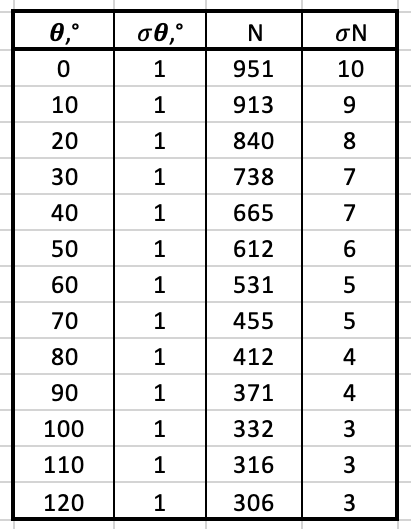
\includegraphics[scale=0.7]{Таблица.PNG}
	\end{figure}

	\item Построим графики зависимости $1/N = f(1-\cos \theta)$:
	
    \[\frac{1}{N(\theta)} - \frac{1}{N(0)} = A(1 - \cos \theta)\]
    
    	\begin{figure}[h!]
	    \centering
		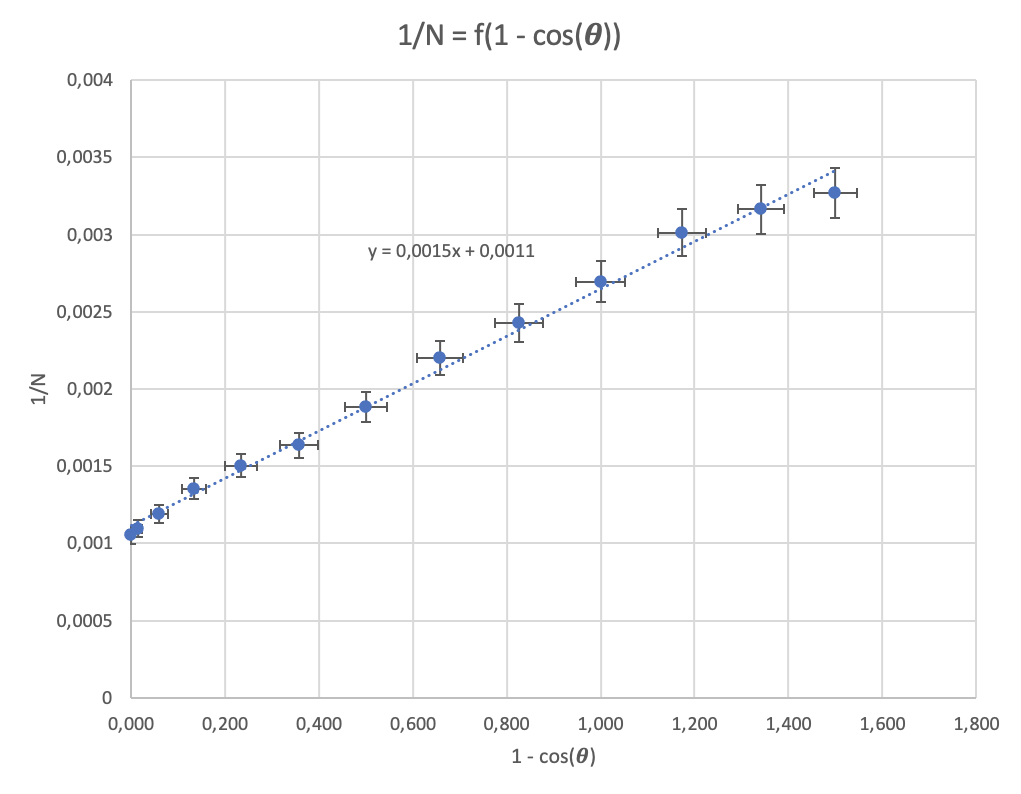
\includegraphics[scale=0.7]{График.PNG}
	\end{figure}

	   \item Посчитаем наилучшие значения $N(0)$ и $N(90)$ для углов $\theta = 0^{\circ}$ и $\theta =90^{\circ}$:

	\[N(0) = 909 \pm 19\]

	\[N(90) = 384 \pm 9\]

	\item Определим энергию покоя электрона: 

	\[mc^2 = E_{\gamma}\dfrac{N(90)}{N(0) - N(90)},\]
	где $E_{\gamma} = 662 \text{ кэВ}$

	Получаем:

	\[mc^2 = 519 \pm 19 \text{ кэВ}\]

\end{enumerate}

\textbf{Вывод:}\\\par

	В ходе работы был измерен энергетический спектр  $\gamma$-квантов,  рассеянных на графите.  Экспериментально был проверен эффект Комптона и правильность теоретических соотношений зависимости энергии рассеяния от угла наблюдения. Также в ходе работы была определена с хорошей точностью энергия покоя электрона:

\[\text{Эксперимент: } 519 \pm 19 \text{ кэВ}\]
\[\text{Теоретическое значение: } 511 \text{ кэВ}\]

\end{document}
